% !TEX root = ../main.tex
%
% ========
\chapter{Particle interferometry}
\label{ch:pi}
% ========
  Two-particle interferometry (also called \textit{femtoscopy}) gives a possibility to investigate space-time characteristics of the particle-emitting source created in heavy ion collisions.
  Through the study of particle correlations, their momentum distributions can be used to obtain information about the spatial extent of the created system.
  Using this method, one can measure sizes of the order of $10^{-15}$ m and time of the order of $10^{-23}$ s.
  %
  % ========
  \section{HBT interferometry}
  % ========
    In the 1956 Robert Hanbury Brown and Richard Q. Twiss proposed a method which allowed to investigate angular dimensions of stars through analysis of interference between photons.
    They performed a measurement of the intensity of a beam of light coming from a star using two separated detectors.
    In a signal plotted as a function of distance between detectors an interference effect was observed, revealing a positive correlation, despite the fact that no phase information was collected.
    Hanbury, Brown and Twiss used this interference signal to calculate the angular size of a star with the excellent resolution.
    This method was designed to be used in astronomy, however HBT interferometry can be used also to measure extent of any emitting source.
    Therefore it was adapted to heavy ion collisions to investigate dimensions of a particle-emitting source~\cite{drkisiel}.
  %
  % ========
  \section{Theoretical approach}
  % ========
    Intensity interferometry in heavy ion physics uses similar mathematical formalism as the astronomy HBT measurement.
    The difference between them is that femtoscopy uses a two-particle relative momentum and yields the space-time picture of a source, whereas the latter method uses the distance between detectors to calculate angular size of the star.
    %
    % ========
    \subsection{Conventions used}
    % ========
      In heavy ion collisions to describe particular directions, components of momentum and location of particles, one uses naming convention called the Bertsch-Pratt coordinate system.
      This system is presented in the Fig.~\ref{fig:coordinate-system}.
      \begin{figure}[h]
        \centering
        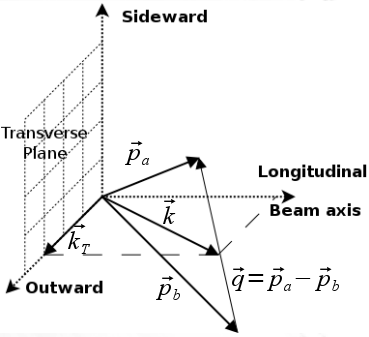
\includegraphics[width=0.5\textwidth]{coordinate_system}
        \caption{Bertsch-Pratt direction naming convention used in heavy ion collision.}
        \label{fig:coordinate-system}
      \end{figure}
      The three directions are called \textit{longitudinal}, \textit{outward} and \textit{sideward}.
      The longitudinal direction is parallel to the beam axis.
      The plane perpendicular to the beam axis is called a \textit{transverse plane}.
      A projection of a particle pair momentum $\vect{k} = (\vect{p}_a + \vect{p}_b)/2$ on a transverse plane (a \textit{transverse momentum} $\vect{k}_T$) determines \textit{outward} direction: $(\vect{k})_{out} = \vect{k}_T$.
      A direction perpendicular to the longitudinal and outward is called \textit{sideward}.

      A particle pair is usually described using two coordinate systems.
      The first one, \textit{Longitudinally Co-Moving System} (\textbf{LCMS}) is moving along the particle pair with the longitudinal direction, in other words, the pair longitudinal momentum vanishes: $(\vect{p}_a)_{long} = -(\vect{p}_b)_{long} $.
      The second system is called \textit{Pair Rest Frame} (\textbf{PRF}).
      In the PRF the centre of mass rests: $\vect{p}_a = -\vect{p}_b$.
      Variables which are expressed in the PRF are marked with a star (e.g. $\vect{k}^{*}$).

      The transition of space-time coordinates from LCMS to PRF is simply a boost along the outward direction, with the transverse velocity of the pair~$\beta_T = (\vect{v}/c)_{out}$~\cite{nonidfemto}:
      \begin{align}
        \label{eq:lcmstoprf}
        r^{*}_{out} &= \gamma_{t}(r_{out} - \beta_T \Delta t)\\
        r^{*}_{side} &= r_{side}\\
        r^{*}_{long} &= r_{long}\\
        \Delta t^{*} &= \gamma_T(\Delta t - \beta_T r_{out})~, 
      \end{align}
      where $\gamma_T = (1-\beta^{2}_T)^{-1/2}$ is the Lorentz factor.
      However, in calculations performed in this work the equal time approximation is used, which assumes that particles in a pair were produced at the same time in PRF - the $\Delta t^{*}$ is neglected.

      The most important variables used to describe particle pair are their total momentum $\vect{P} = \vect{p}_a + \vect{p}_b$ and relative momentum $\vect{q} = \vect{p_a} - \vect{p_b}$.
      In the PRF one has $\vect{q} = 2 \vect{k}^{*}$, where $\vect{k}^{*}$ is a momentum of the first particle in PRF.

    %
    % ========
    \subsection{Two particle wave function}
    % ========
      Let us consider two identical particles with momenta $\vect{p_1}$ and $\vect{p_2}$ emitted from space points $\vect{x_1}$ and $\vect{x_2}$.
      Those emitted particles can be treated as two incoherent waves.
      \begin{figure}[h]
        \centering
        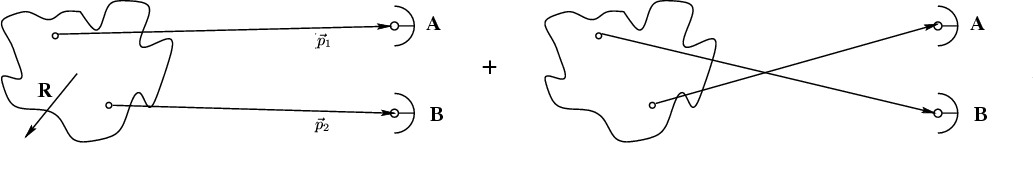
\includegraphics[width=0.9\textwidth]{wavefunction}
        \caption{The pair wave function is a superposition of all possible states. In case of particle interferometry it includes two cases: particles with momenta $p_1$,~$p_2$ registered by detectors \textit{A}, \textit{B} and $p_1$,~$p_2$ registered by \textit{B}, \textit{A} respectively.}
        \label{fig:wavefunction}
      \end{figure}
      If the particles are identical, they are also indistinguishable, therefore one has also take into account the scenario, where the particle with momentum $\vect{p_1}$ is emitted from $\vect{x_2}$ and particle $\vect{p_2}$ from $\vect{x_1}$ (Fig.~\ref{fig:wavefunction}).
      In such case, the wave function describing behaviour of a pair has to contain both components~\cite{drkisiel}:
      \begin{equation}
      \label{eq:wavefunction}
        \Psi_{ab}(\vect{q})=\frac{1}{\sqrt{2}} \left[ \exp(- i \vect{p_1}\vect{x_1} - i \vect{p_2}\vect{x_2}) \pm \exp(- i \vect{p_2}\vect{x_1} - i \vect{p_1}\vect{x_2}) \right]~.
      \end{equation}
      A two particle wave function of identical bosons is symmetric (``+'' sign in Eq.~\ref{eq:wavefunction}) and in case of identical fermions - antisymmetric (``-'' sign).
      This anti-symmetrization or symmetrization implies the correlation effect coming from the Fermi-Dirac or Bose-Einstein statistics accordingly.

      To provide full description of a system consisting of two charged hadrons, one has to include in the wave function besides quantum statistics also Coulomb and strong Final State Interactions.
      The aim of this work is an analysis of femtoscopic radii proportional to the inverse of a width of a correlation function (for detailed description see Section~\ref{sec:correlation-function}).
      Since we are not interested in the direct comparison of experimental correlation functions with their analytical forms, the following simplification can be made.
      A width of identical particles correlation function is determined by effects coming from quantum statistics, hence one can ignore influence of Final State Interactions, which in this case is small. Taking into account only quantum statistics can reduce complexity of calculations and save computation time.
    %
    % ========
    \subsection{Source emission function}
    % ========
      To describe particle emitting source, one uses a single emission function~\cite{nonidfemto}:
      \begin{equation}
        \label{eq:source-single-3d}
        S_A(\vect{x}_1,\vect{p}_1) = \int S(\vect{x}_1,\vect{p}_1,\vect{x}_2,\vect{p}_2,...,\vect{x}_N,\vect{p}_N)
        d \vect{x}_2 d \vect{p}_2 ... d \vect{x}_N d \vect{p}_N
      \end{equation}
      and a two-particle one:
      \begin{equation}
        \label{eq:source-two-3d}
        S_{AB}(\vect{x}_1,\vect{p}_1,\vect{x}_2,\vect{p}_2) = \int S(\vect{x}_1,\vect{p}_1,\vect{x}_2,\vect{p}_2,...,\vect{x}_N,\vect{p}_N)
        d \vect{x}_3 d \vect{p}_3 ... d \vect{x}_N d \vect{p}_N~.
      \end{equation}
      Emission function $S(\cdot)$ can be interpreted as a probability to emit a particle, or a pair of particles from a given space-time point with a given momentum.
      In principle, the source emission function should encode all physics aspects of the particle emission process i.e. the symmetrization for bosons and fermions, as well as the two-body and many body Final State Interactions.
      Instead of this, one assume that each particle's emission process is independent - the interaction between final-state particles after their creation is independent from their emission process.
      The assumption of this independence allows to construct two-particle emission function from single particle emission functions via a convolution~\cite{nonidfemto}:
      \begin{equation}
        \label{eq:source-two-conv}
        \begin{split}
          S(\vect{k}^{*},\vect{r}^{*}) = \int S_A ( \vect{p}_1, \vect{x}_1 ) S_B ( \vect{p}_2, \vect{x}_2 )
          \delta \left[\vect{k}^{*} - \frac{\vect{p}_1+\vect{p}_2}{2} \right]
          \delta \left[\vect{r}^{*} - (\vect{x}_1+\vect{x}_2) \right] \\
          \times~d^4 \vect{x}_1 d^4 \vect{x}_2 d^4 \vect{x}_1 d^3 \vect{p}_1 d^3 \vect{p}_2
        \end{split}
      \end{equation}
      In case of identical particles, ($S_A = S_B$) several simplifications can be made.
      A convolution of the two identical Gaussian distributions is also a Gaussian distribution with $\sigma$ multiplied by $\sqrt{2}$.
      Femtoscopy can give information only about two-particle emission function, but when considering Gaussian distribution as a source function in Eq.~\ref{eq:source-two-conv}, one can obtain a $\sigma$ of a single emission function from a two-particle emission function.
      The Eq.~\ref{eq:source-two-conv} is not reversible - an information about $S_A(\cdot)$ cannot be derived from $S_{AB}(\cdot)$.
      An exception from this rule is a Gaussian source function, hence it is often used in femtoscopic calculations.
      Considering pairs of identical particles, an emission function is assumed to be described by the following equation in the Pair Rest Frame~\cite{nonidfemto}:
      \begin{equation}
        S^{PRF}_{1D} (\vect{r}^{*}) = \exp \left( - \frac{ {r_{out}^*}^{2} + {r_{side}^*}^{2} + {r_{long}^*}^{2}}{4 {R_{inv}}^2} \right)~.
      \end{equation}
      To change from the three-dimensional variables to the one-dimensional variable one requires introduction of the proper Jacobian~${r^*}^2$:
      \begin{empheq}[innerbox=\fbox, right=~.]{align}
        \label{eq:source-1d-prf}
        S^{PRF}_{1D} (r^{*}) = {r^*}^{2} \exp \left( - \frac{{r^*}^{2}}{4 {R_{inv}}^2} \right)
      \end{empheq}
      The ``4'' in the denominator before the ``standard deviation'' $R_{inv}$ in the Gaussian distribution comes from the convolution of the two Gaussian distributions, which multiplies the $R_{inv}$ by a factor of $\sqrt{2}$.

      A more complex form of emission function was used by all RHIC and SPS experiments in identical pion femtoscopy:
      \begin{empheq}[innerbox=\fbox, right=~.]{align}
        \label{eq:source-3d-lcms}
        S^{LCMS}_{3D} (\vect{r}) = \exp \left( 
          - \frac{ r_{out}^{2}}{4 {R_{out}}^2}
          - \frac{ r_{side}^{2}}{4 {R_{side}}^2}
          - \frac{ r_{long}^{2}}{4 {R_{long}}^2}
        \right)
      \end{empheq}
      The main difference of this source function is that it has three different and independent widths $R_{out}$, $R_{side}$, $R_{long}$ and they are defined in the LCMS, not in PRF.
      Unlike in PRF, in LCMS an equal-time approximation is not used.
      For identical particles this is not a problem - only Coulomb interaction inside a wave function depends on $\Delta t$.
      %
      % ========
      \subsubsection{Relationship between one-dimensional and three-dimensional source sizes}
      % ========
      Up to now, most of femtoscopic measurements were limited only to averaged source size $R^L_{av}$ (the letter ``L'' in superscript stands for LCMS):
      \begin{equation}
        S^{LCMS}_{1D} (\vect{r}) = \exp \left( - \frac{ {r_{out}}^{2} + {r_{side}}^{2} + {r_{long}}^{2}}{2 {R^{L}_{av}}^2} \right)~.
      \end{equation}
      The relationship between between $S^{LCMS}_{1D}(\cdot)$ and $S^{LCMS}_{3D}(\cdot)$ is given by:
      \begin{equation}
        \begin{split}
        \label{eq:source-1d-from-3d}
        S^{LCMS}_{3D} (r) = \int \exp \left( 
          - \frac{ r_{out}^{2}}{2 {R^L_{out}}^2}
          - \frac{ r_{side}^{2}}{2 {R^L_{side}}^2}
          - \frac{ r_{long}^{2}}{2 {R^L_{long}}^2}
        \right)
        \\ \times~\delta \left(
          r - \sqrt{ r_{out}^{2} + r_{side}^{2} + r_{long}^{2}}
        ~\right)
        d r_{out} d r_{side} d r _{long}~.
        \end{split}
      \end{equation}
      The one-dimensional source size corresponding to the three-dimensional one can be approximated by the following form:
      \begin{equation}
        \label{eq:source-1d-lcms}
        S^{LCMS}_{1D} (r) = {r}^{2} \exp \left( - \frac{r^{2}}{2 {R^L_{av}}^2} \right)~.
      \end{equation}
      The equation above assumes that $R^L_{out} = R^L_{side} = R^L_{long}$ hence $R^L_{av} = R^L_{out}$.
      \begin{figure}[h]
        \centering
        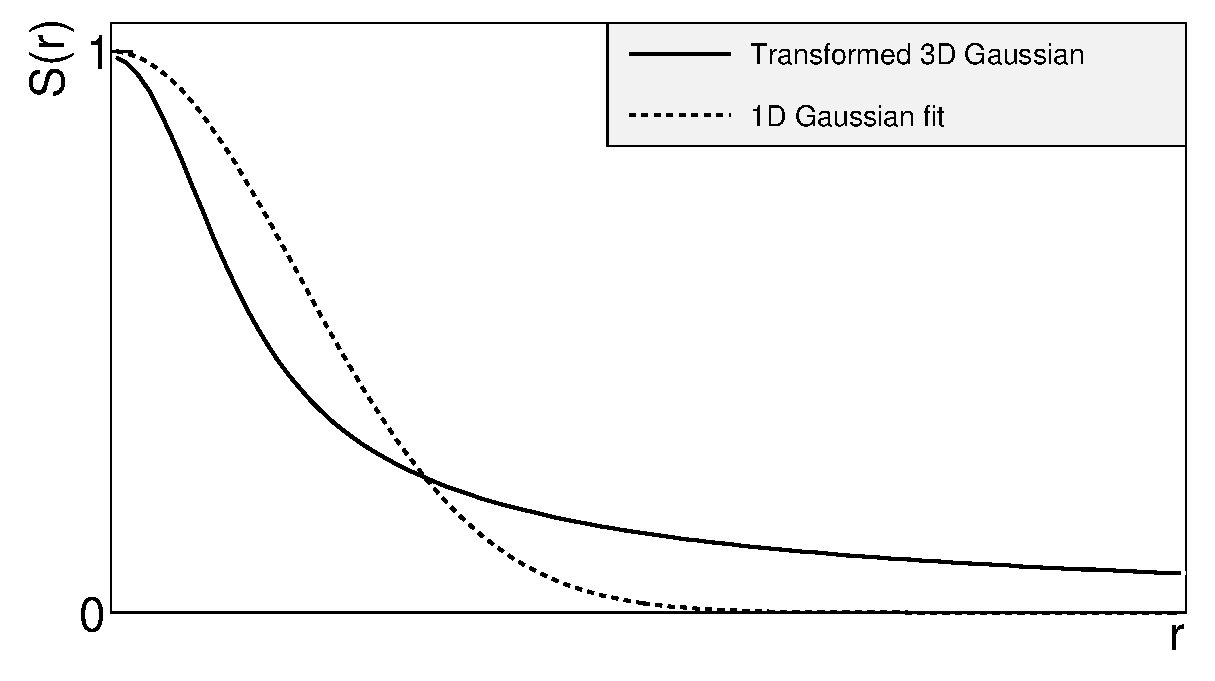
\includegraphics[width=0.7\textwidth]{3dg21d}
        \caption{An averaged three-dimensional Gaussian source function with different widths was averaged into one-dimensional function. To illustrate deformations, one-dimensional Gaussian distribution was fitted.}
        \label{fig:3dgaussian}
      \end{figure}
      If this condition is not satisfied, one can not give explicit mathematical relation between one-dimensional and three-dimensional source sizes.
      However, for realistic values of $R$ (i.e. for similar values of $R_{out}$, $R_{side}$, $R_{long}$), the $S^{LCMS}_{3D}$ from Eq.~\ref{eq:source-1d-from-3d} is not very different from Gaussian distribution and can be well approximated by Eq.~\ref{eq:source-1d-from-3d}.

      A deformation of an averaged source function in case of big differences in $R_{out}$, $R_{side}$, $R_{long}$ is presented in the Fig.~\ref{fig:3dgaussian}.
      A three-dimensional Gaussian distribution with varying widths was averaged into one-dimensional function using the Eq.~\ref{eq:source-1d-from-3d}.
      Afterwards, an one-dimensional Gaussian distribution was fitted.
      One can notice a heavy tail of an averaged distribution in long $r$ region, which makes an approximation using one-dimensional distribution in this case quite inaccurate.
      
      Using Eq.~\ref{eq:source-1d-from-3d} and Eq.~\ref{eq:source-1d-lcms} one can obtain a relation between one-dimensional width and the three-dimensional ones.
      Through numerical calculations one can find the following approximate relation~\cite{nonidfemto}:
      \begin{empheq}[innerbox=\fbox, right=~.]{align}
        R^{L}_{av} = \sqrt{ \left. \left( {R^L_{out}}^2 + {R^L_{side}}^2 + {R^L_{long}}^2 \right) \middle/ 3 \right. }
      \end{empheq}
      This equation does not depend on the pair velocity, hence it is valid in the LCMS and PRF.
    %
    % ========
    \subsection{Analytical form of a correlation function}
    \label{sec:correlation-function}
    % ========
      The fundamental object in a particle interferometry is a correlation function.
      The correlation function is defined as:
      \begin{equation}
        \label{eq:th_cf}
        C(\vect{p}_a,\vect{p}_b) = \frac{P_2(\vect{p}_a,\vect{p}_b)}{P_1(\vect{p}_a) P_1(\vect{p}_b)}~,
      \end{equation}
      where $P_2$ is a conditional probability to observe a particle with momentum $\vect{p}_b$ if particle with momentum $\vect{p}_a$ was also observed.
      A $P_1$ is a probability to observe a particle with a given momentum.
      The relationship between source emission function, pair wave function and the correlation function is described by the following equation:
      \begin{equation}
        \label{eq:cf_integral}
        C(\vect{p}_1,\vect{p}_2) = \int S_{AB}(\vect{p}_1,\vect{x}_1,\vect{p}_2,\vect{x}_2)
          |\Psi_{AB}|^2 d^4 \vect{x}_1 d^4 \vect{x}_2
      \end{equation}
      Substituting the one-dimensional emission function (Eq.~\ref{eq:source-1d-prf}) into the integral above yields the following form of correlation function in PRF:
      \begin{empheq}[innerbox=\fbox, right=~,]{align}
        \label{eq:cf_1d}
        C(q) = 1 + \lambda \exp \left( - R_{inv}^2 q^2 \right)
      \end{empheq}
      where $q$ is a momentum difference between two particles.
      When using the three-dimensional emission function (Eq.~\ref{eq:source-3d-lcms}) one gets the following correlation function defined in the LCMS:
      \begin{empheq}[innerbox=\fbox, right=~,]{align}
        C(\vect{q}) = 1+ \lambda \exp \left( -R_{out}^2 q_{out}^2 -R_{side}^2 q_{side}^2 -R_{long}^2 q_{long}^2  \right)
      \end{empheq}
      where $q_{out}$, $q_{side}$, $q_{long}$ are $\vect{q}$ components in the outward, sideward and longitudinal direction.
      The $\lambda$ parameter in the equations above determines correlation strength.
      The lambda parameter has values in the range $\lambda \in [-0.5,1]$ and it depends on a pair type.
      In case of pairs of identical bosons (like $\pi$-$\pi$ or $K$-$K$) the lambda parameter $\lambda \to 1$. For identical fermions (e.g. $p$-$p$) $\lambda \to$~-0.5.
      Values of $\lambda$ observed experimentally are lower than 1 (for bosons) and greater than -0.5 (for fermions).
      There are few explanations to this effect: detector efficiencies, inclusion of misidentified particles in a used sample or inclusion of non-correlated pairs (when one or both particles come from e.g. long-lived resonance).
      The analysis carried out in this work uses data from a model, therefore the detector efficiency and particle purity is not taken into account~\cite{nonidfemto}.
    %
    % ========
    \subsection{Spherical harmonics decomposition of a correlation function}
    % ========
      Results coming from an analysis using three-dimensional correlation function in Cartesian coordinates are quite difficult to visualize.
      To do that, one usually performs a projection into one dimension in outward, sideward and longitudinal directions. 
      One may loose important information about a correlation function in this procedure, because it gives only a limited view of the full three-dimensional structure.
      Recently, a more advanced way of presenting correlation function - a spherical harmonics decomposition, was proposed.
      The three-dimensional correlation function is decomposed into an infinite set of components in a form of one-dimensional histograms $C^m_l (q)$.
      In this form, a correlation function is defined as a sum of a series~\cite{sh}:
      \begin{equation}
        C(\vect{q}) = \sum_{l,m} C^m_l (q) Y^m_l(\theta, \phi)~,
      \end{equation}
      where $Y^m_l(\theta,\phi)$ is a spherical harmonic function.
      Spherical harmonics are an orthogonal set of solutions to the Laplace's equation in spherical coordinates
      Hence, in this approach, a correlation function is defined as a function of $q$, $\theta$ and $\phi$.
      To obtain $C^m_l$ coefficients in the series, one has to calculate the following integral:
      \begin{equation}
        \label{eq:sh_decomposition}
        C^m_l(q) = \int_\Omega C(q,\theta,\phi) Y^{m*}_l (\theta,\phi) d \Omega~,
      \end{equation}
      where $\Omega$ is a full solid angle.

      Spherical harmonics representation has several important advantages.
      The main one is that it requires less statistics than traditional analysis performed in Cartesian coordinates.
      Another one is that it encodes full three-dimensional information in a set of one-dimensional plots. 
      In principle it does not have to be an advantage, because full description of a correlation function requires infinite number of \textit{l}, \textit{m} components.
      But it so happens that the intrinsic symmetries of a pair distribution in a femtoscopic analysis result in most of the components to vanish.
      For the identical particles correlation functions, all coefficients with odd values of \textit{l} and \textit{m} disappear.
      % Because the values of a correlation function are real, the imaginary part of a series are equal to zero ($\Im C^m_l = 0$).
      It has also been shown, that the most significant portion of femtoscopic data is stored in the components with the lowest \textit{l} values.
      It is expected that, the main femtoscopic information is contained in the following components~\cite{nonidfemto}:
      \begin{align}
        C^0_0 &\to R_{LCMS}~, \\
        \Re C^0_2 &\to \frac{R_T}{R_{long}}~, \\
        \Re C^2_2 &\to \frac{R_{out}}{R_{side}}~,
      \end{align}
      where $R_{LCMS} = \sqrt{ \left. \left( {R_{out}}^2 + {R_{side}}^2 + {R_{long}}^2 \right) \middle/ 3 \right. }$ and $R_{T} = \sqrt{ \left. \left( R_{out}^2 + R_{side}^2 \right) \middle/2 \right. }$.
      The $C^0_0$ is sensitive to the overall size of a correlation function.
      The $\Re C^0_2$ carries the information about the ratio of the transverse to the longitudinal radii, due to its $\cos^2(\theta)$ weighting in $Y^0_2$.
      The component $\Re C^2_2$ with its $\cos^2(\phi)$ weighting encodes the ratio between outward and sideward radii.
      Thus, the spherical harmonics method allows to obtain and analyze full three-dimensional femtoscopic information from a correlation function~\cite{nonidfemto}.

  %
  % ========
  \section{Experimental approach}
  % ========
    The correlation function is defined as a probability to observe two particles together divided by the product of probabilities to observe each of them separately (Eq.~\ref{eq:th_cf}). 
    Experimentally this is achieved by dividing two distributions of relative momentum of pairs of particles coming from the same event and the equivalent distribution of pairs where each particle is taken from different collisions.
    In this way, one obtains not only femtoscopic information but also all other event-wide correlations.
    This method is useful for experimentalists to estimate the magnitude of non-femtoscopic effects.
    There exists also a different approach, where two particles in pairs in the second distribution are also taken from the same event.
    The second method gives only information about physical effects accessible via femtoscopy.
    The aim of this work is a study of effects coming from two particle interferometry, hence the latter method was used. 

    In order to calculate experimental correlation function, one uses the following approach.
    One has to construct two histograms: the \textit{numerator} $N$ and the \textit{denominator} $D$ with the particle pairs momenta, where particles are coming from the same event.
    Those histograms can be one-dimensional (as a function of $|\vect{q}|$), three dimensional (a function of three components of $\vect{q}$ in LCMS) or a set of one-dimensional histogram representing components of the spherical harmonic decomposition of the distribution.
    The second histogram, $D$ is filled for each pair with the weight 1.0 at a corresponding relative momentum $\vect{q} = 2 \vect{k^*}$.
    The first one, $N$ is filled with the same procedure, but the weight is calculated as $|\Psi_{ab}(\vect{r^*},\vect{k^*})|^2$.
    A division $N/D$ gives the correlation function $C$.
    This procedure can be simply written as~\cite{nonidfemto}:
    \begin{equation}
      % C(\vect{k^*}) = \frac{N}{D} =  \frac{\int d D(\vect{r^*, k^*}) |\Psi_{ab}(\vect{r^*},\vect{k^*})|^2}{\int d D(\vect{r^*, k^*})}~,
      \label{eq:cf_experimental}
      C(\vect{k^*}) = \frac{N}{D} =  \frac{\sum\limits_{n_i \in D} \delta(\vect{k^*}_i - \vect{k^*}) |\Psi_{ab}(\vect{r^*}_i,\vect{k^*}_i)|^2 }{\sum\limits_{n_i \in D} \delta(\vect{k^*}_i - \vect{k^*})}~.
    \end{equation}
    The $D$ histogram represents the set of all particle pairs used in calculations.
    The~$n_i$ is a pair with the its relative momentum $\vect{k^*}_i$ and relative separation $\vect{r^*}_i$.
    Mathematically, the procedure of calculating the Eq.~\ref{eq:cf_experimental} is equivalent to a calculation of an integral in Eq.~\ref{eq:cf_integral} through a Monte-Carlo method.
    The~wave function used in Eq.~\ref{eq:cf_experimental} has one of the following forms:
    \begin{align}
      |\Psi_{\pi\pi}(\vect{r^*},\vect{k^*})|^2 = |\Psi_{KK}(\vect{r^*},\vect{k^*})|^2 &= 1 + \cos(2 \vect{k^*} \vect{r^*})~, \\
      \label{eq:pp-wf}
      |\Psi_{pp}(\vect{r^*},\vect{k^*})|^2 &= 1 - \frac{1}{2} \cos(2 \vect{k^*} \vect{r^*})~.
    \end{align}
    The first one is used in case of bosons, and the latter one is for identical fermions.
    A wave function for pair of spin-1/2 fermions (Eq.~\ref{eq:pp-wf}) is a superposition of two possible states: singlet state (with spin equal to 0 and one eigenstate) and triplet state (with spin equal to 1 and three possible eigenstates).
    For a singlet state, a wave function is symmetric, and for triplet state, it is antisymmetric.
    In other words the $|\Psi_{pp}|^2$ encodes correlation coming from Bose-Einstein statistics (with weight $1/4$) and anti-correlation from Fermi-Dirac distribution (with weight $3/4$).
    % the coefficient before cosine in the $|\Psi_{pp}|^2$ is equal to \mbox{$(-1) \times 3/4 + 1 \times 1/4 = -1/2$}.
  % include drkisiel p. 35?
  % 1D vs 3D

  %
  % ========
  \section{Scaling of femtoscopic radii}
  \label{ch:pi-scaling}
  % ========
    A particle interferometry formalism presented in the previous sections assumes that particle emitting source is static.
    This is not the case in heavy ion collisions at LHC.
    An existence of transverse radial and elliptic flow suggest that created system is dynamic.
    To address this issue, a concept of \textit{lengths of homogeneity} was introduced.
    It is defined as:
    \begin{equation}
      \frac{|f(p,x + \lambda) - f(p,x)|}{f(p,x)} = 1~,
    \end{equation}
    where $\lambda$ is the homogeneity length.
    It can be interpreted as the distance at which relative change of the source Wigner function $f$ becomes large.
    One can measure the lengths of homogeneity of a system using femtoscopic radii.
    This concept can be intuitively explained on a basis of hydrodynamic models.
    Each source element is emitting particles with a velocity which is a combination of two components: a fluid cell velocity $\beta_f$ (which is taken from the flow field $u_{\mu}(\vect{x^{\mu}})$) and thermal velocity $\beta_{th}$ (which has random direction).
    These particles can combine into pairs of small relative momenta and become correlated.
    If two particles are emitted far ($|\vect{x}_a - \vect{x}_b| > \lambda$) away from each other, the flow field $u_\mu$ in their point of emission might be very different and it will be impossible for them to have sufficiently small relative momenta to be in the region of interference effect.
    This effect is presented in Fig.~\ref{fig:cf_width}.
    An increase of a correlation is visible for pairs with low relative momenta~\cite{drkisiel}.
    % In the hydrodynamic models describing expansion of a quark-gluon plasma, particles are emitted from the source elements.
    % Each of the source elements is moving with the velocity $u_\mu$ given by hydrodynamic equations.
    % Because solutions of those equations are smooth, nearby source elements have similar velocities.
    % Each emitted particle from a certain source element is boosted with the flow velocity $u_\mu$ according to the point of origin.
    \begin{figure}[h]
      \centering
      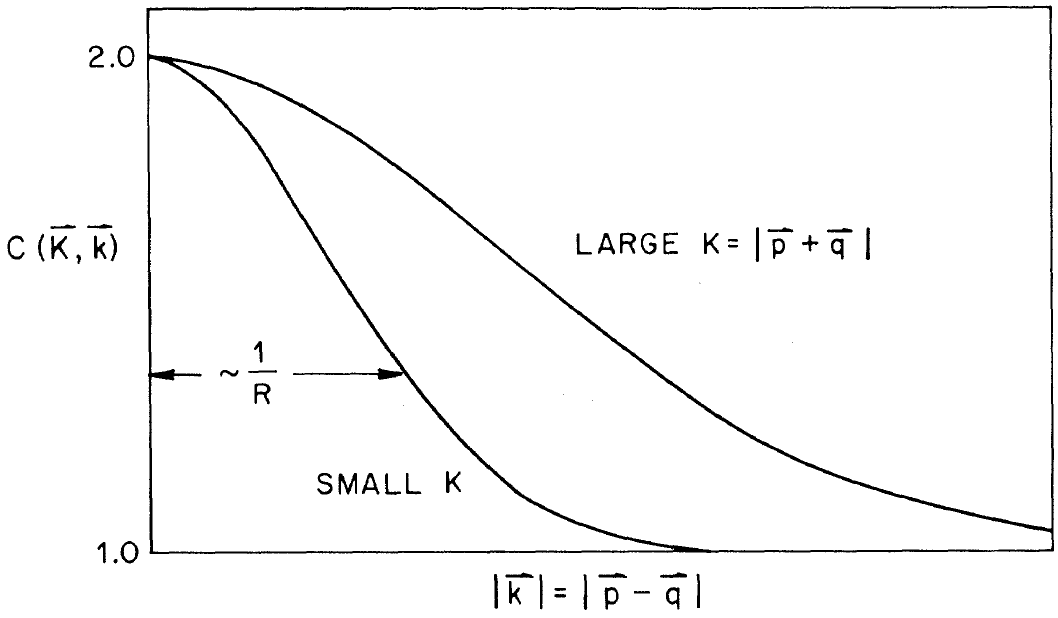
\includegraphics[width=0.7\textwidth]{cf_width_dep}
      \caption{Correlation function width dependence on total pair momentum. Pion pairs with a large total momentum have a wider correlation (smaller apparent source)~\cite{pratt_pion}.}
      \label{fig:cf_width}
    \end{figure}
    % Hence particles emitted close to each other (pairs with large transverse momentum $|\vect{k}_T|$) will gain the similar velocity boost, they can combine into pairs with small relative momenta ($|\vect{q}|$) and therefore become correlated.
    % If the two particles are emitted far away from each other (a pair with small $|\vect{k}_T|$), the flow field $u_\mu$ in their point of emission might be very different and it will be impossible for them to have sufficiently small relative momenta in order to be in region of interference effect.
    % This effect is visible in a width of a correlation function in the Fig.~\ref{fig:cf_width}.
    % The correlation function gets broader for greater values of $|\vect{k}_T|$ and the femtoscopic radius $R$ becomes smaller~\cite{drkisiel,pratt_pion}.
    %
    % ========
    \subsection{Scaling in LCMS}
    % ========
      Hydrodynamic calculations performed in LCMS show that femtoscopic radii in outward, sideward, and longitudinal direction show dependence on transverse mass $m_T~=~\sqrt{k^2_T + m^2}$, where $m$ is a mass of a particle~\cite{akkelin_sinyukov}.
      Moreover, experimental results show  that this scaling is observed for $R_{LCMS}$ radii also.
      This dependence can be expressed as follows:
      \begin{empheq}[innerbox=\fbox, right=~,]{align}
        \label{eq:r_scaling}
        R_i = \alpha m_T^{-\beta}
      \end{empheq}
      where $i$ subscript indicates that this equation applies to $R_{out}$, $R_{side}$ and $R_{long}$ radii.
      The $\beta$ exponent is approximately equal 0.5.
      In case of strong transversal expansion of the emitting source, the decrease of longitudinal interferometry radius can be more quick than $m_T^{-0.5}$, hence one can expect for longitudinal radii greater values of $\beta >$~0.5~\cite{akkelin_sinyukov}.
      % \/ do wynikow
      % the scaling behavior shows that hydro produces common collective behavior in both transverse dimensions
    %
    % ========
    \subsection{Scaling in PRF}
    % ========
      In the collisions at the LHC energies, pions are most abundant particles and their multiplicities are large enough to enable three-dimensional analysis.
      However, for heavier particles, such as kaons and protons statistical limitations arise.
      Hence it is often possible to only measure one-dimensional radius $R_{inv}$ for those particles.
      The $R_{inv}$ is then calculated in the PRF.
      The transition from LCMS to PRF is a Lorentz boost in the direction of pair transverse momentum with velocity $\beta_T = p_T / m_T$.
      Hence only $R_{out}$ radius changes:
      \begin{equation}
        R_{out}^* = \gamma_T R_{out}~.
      \end{equation} 
      The one-dimensional $R_{inv}$ radius is direction-averaged source size in PRF.
      One can notice, that such power-law scaling of $R_{inv}$ described by Eq.~\ref{eq:r_scaling} is not observed.
      To recover such scaling in PRF one has to take into consideration two effects when transforming variables from LCMS to PRF: overall radius growths and source distribution becomes non-Gaussian, while developing long-range tails (see Fig.~\ref{fig:3dgaussian} for an example).
      The interplay of these two effects can be accounted with an approximate formula:
      \begin{equation}
        R_{inv} = \sqrt{ \left. \left( {R_{out}}^2\sqrt{\gamma_T} + {R_{side}}^2 + {R_{long}}^2 \right) \middle/ 3 \right. }~.
      \end{equation}
      Assuming that all radii are equal $R_{out} = R_{side} = R_{long}$ this formula can be simplified:
      \begin{empheq}[innerbox=\fbox, right=~.]{align}
        R_{LCMS} \approx R_{inv} \times \left[ \left. \left( \sqrt{\gamma_T} + 2 \right) \middle/ 3 \right. \right]^{-1/2}
      \end{empheq}
      This approximate formula allows to restore power-law behaviour of the scaled radii not only when the radii are equal, but also when their differences are small (for explanation see the last part of the section~3.2.3).

      This method of recovering scaling in PRF can be used as a tool for the search of hydrodynamic collectivity between pions, kaons and protons in heavy ion collisions with the measurement of one-dimensional radius in PRF.
